\begin{savequote}[75mm] 
Knowing is not enough; we must apply. Willing is not enough; we must do
\qauthor{Goethe} 
\end{savequote}

\chapter{Use Cases} \label{section:use_cases}

\newthought{PINV has been used in several research projects}. The following are the study cases that we are most familiar with, and although the research in the presented cases belongs to independent projects, we consider that it is relevant to introduce them to illustrate how PINV can be used to explore and visualise heterogeneous datasets. 

The cases below also serve to trace the evolution that the tool has experienced since its conception. The first two use cases listed below were research projects carried out in the same group where PINV was developed, the first of which exposed the need for a tool such as PINV and serve to define the original requirements of PINV. With the second research project, these requirements were polished and finalised.  The third research project mentioned below is the first independent research that used PINV to explore their data and visualise their results. We got direct feedback from users, which helped us to resolve many bugs and to implement new features. The use of PINV's collaborative functions proved to be vital with the progression of this international collaboration. Lastly we present a study where the volume of data was bigger than previous datasets, which was used to test some of the server capabilities, and it is used here to show the potential of the spatial clustering technique.

\section{Predicting and Analyzing Interactions between \emph{Mycobacterium tuberculosis} and Its Human Host} \label{sec:mb_human}

\begin{figure}
\centering
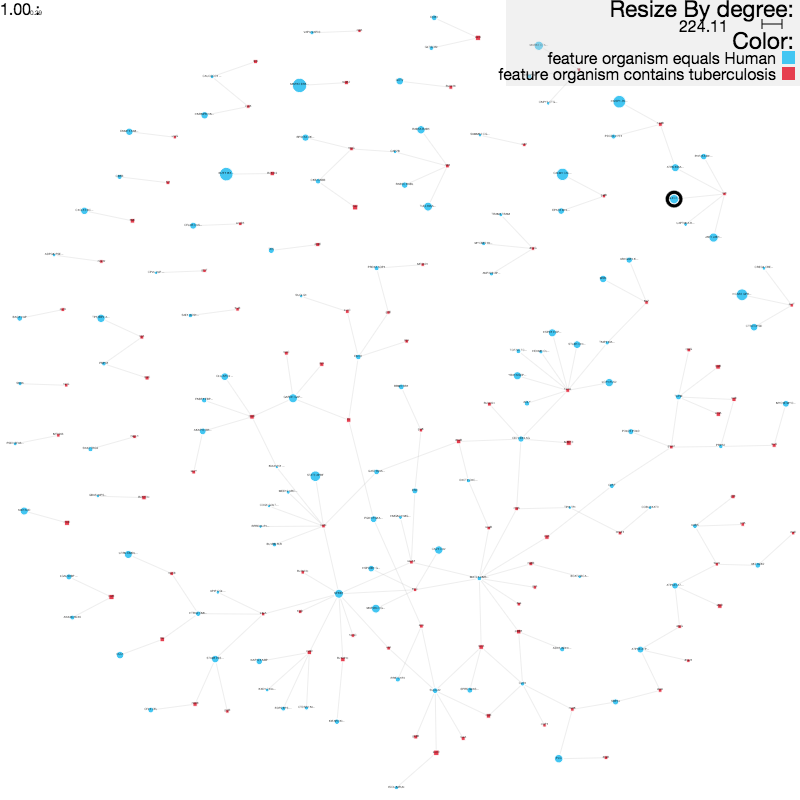
\includegraphics[width=\textwidth]{figures/pinv_human_mtb.png}
\caption[Predicted functional interactions between MTB and Human]{Predicted functional interactions between MTB and Human. Blue circles are human proteins while red squares are from the MTB microorganism.
\label{fig:pinv_human_mtb}}
\end{figure}

\subsection{Research description}
This research is based on the fact that diseases such as tuberculosis are better understood from the relationships between the pathogens and their host. Some of these relationships can be described as protein-protein interactions, where one protein belongs to the microorganism and the other to the host. Such interactions are not required to be direct (i.e proteins binding to each other), and can be what is known as a functional interaction, where, for instance,  the presence of one protein has an effect on the function of another protein. 

Although highly relevant to the understanding of several biological processes, experimental studies of host-pathogen protein interactions are very scarce, and therefore computational prediction is the available alternative. In this study, the authors used the interologs method in order to predict functional interactions between \emph{Mycobacterium tuberculosis} (MTB) and \emph{Homo sapiens}. The predicted interactions were filtered by selecting only those differently expressed during infection. The resulting set was then validated based on the known location of the proteins in the cell, verifying that they belong to an area where cross-organism interaction is actually possible. 

The 190 proteins found were further analysed using functional and metabolical pathway knowledge, confirming the potential for some of these proteins to be drug targets \cite{RAP2013}. These interactions also illustrate how MTB might acquire nutrients and how it modulates the host response to its advantage.

Figure \ref{fig:pinv_human_mtb} displays the interactions found in this research project using PINV.


\subsection{Impact on PINV}

When the first results of this research were presented in a group meeting, the authors expressed the difficulties experienced while exploring the interaction datasets, especially when trying to generate visualisations that would help them to explain their findings. Given our experience with the visualisation projects described in section \ref{section:dasvisual} we took up the challenge of developing a tool that can support research projects that deal with this type of data on the web. 

Periodical meetings with the authors of this research helped us to define the requirements of PINV and other methods to improve the user experience of researchers dealing with protein-protein interaction data. 

The first observation from those meetings was that PINV needed to be more an exploratory tool than a graphic generator or an analysis application. This led to the decision to have a repository that can be queried in order to extract only the information of interest, instead of loading the whole network in the visualiser, which ultimately would require the user to preprocess the data with a separate tool.

\begin{figure}
\centering
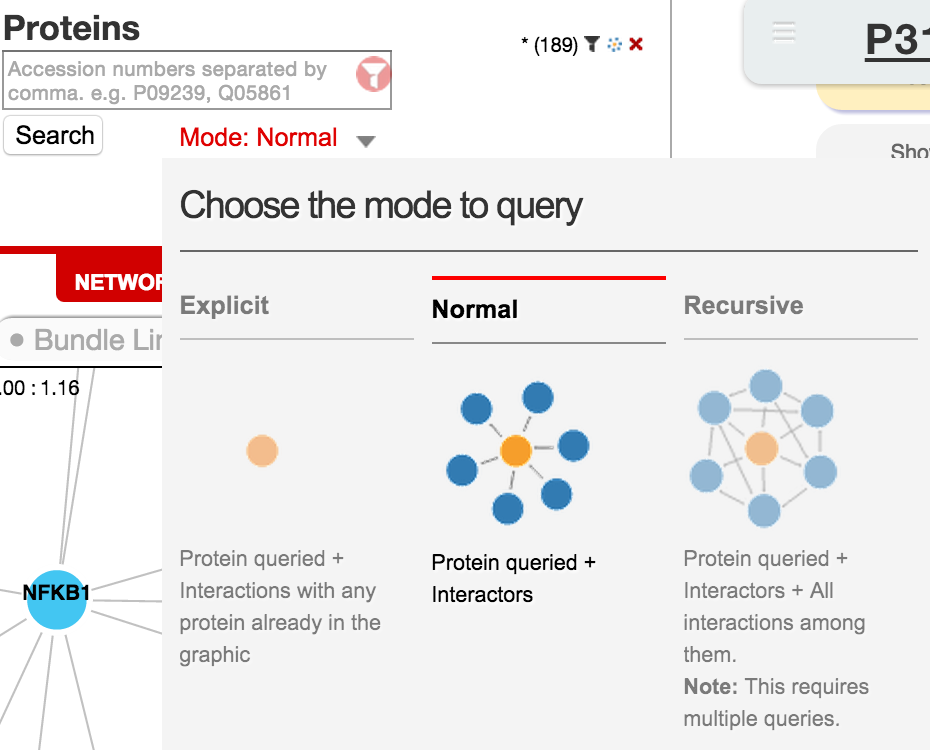
\includegraphics[width=4in]{figures/pinv_modes_query.png}
\caption[Three modes to query by ID in PINV]{Three modes to query by ID in PINV: Explicit, Normal and Recursive
\label{fig:pinv_modes_query}}
\end{figure}

It was with the help of our collaborators that we defined the three modes to query by ID (Figure \ref{fig:pinv_modes_query}). PINV's first versions only included the normal mode in which a queried protein ID retrieves all the interactions where that protein ID has been reported, but later it was pointed out that researchers some times prefer to limit their view to only a subset of proteins. We therefore developed the explicit mode to satisfy this requirement, and later the recursive mode was also added as a combination of the previous two options, allowing the user to obtain all the neighbours of a protein together with the interactions between them.

Another outcome from these meetings was related to the data itself: on the one hand, most of the interaction datasets have similarities -  interaction data is  limited to the definition of pairs of biological molecules, and information about the origin of the interaction is usually restricted to the method used to discover it. On the other hand, the protein data its heterogeneous - each project selects different features to consider, for some, network intrinsic annotations (e.g. degree, closeness, etc.) are the features to consider, while for others, biological features are more relevant (e.g. functional class, cellular location, etc.). 

Based on this, we determined that the upload of data to PINV requires two files: one defining the network with all the interactions between proteins and a second file with the annotations of interest for those proteins. A consequence of this open schema for protein data is that PINV widgets had to adapt to the specificities of each dataset. For example the definition of rules to manipulate the graphic representation considers the features defined for each project, figure \ref{fig:pinv_human_mtb} for instance, uses the degree (i.e. number of connections in the network) of each protein to resize it. Thanks to this, it is easy to identify highly connected proteins, even when the current visualisation is filtering out most of the other connections.

One more requirement gathered at this stage was to support direct manipulation of the visualisation: layouts are of great help to start analysing a network, however the researcher often needs to reorganise the network and manually locate some proteins in order to make  certain characteristics in the graphic more evident. Therefore, proteins in PINV can be moved by dragging them around the graphic, and the simulation forces can be stopped at any time.


\section{Orthologs in 3 Mycobacterial Organisms}\label{sec:orthologs}
\subsection{Research description}
This project presented a comparison between the functional networks of three related microorganisms: \emph{Mycobacterium tuberculosis} (MTB), \emph{Mycobacterium leprae} (MLP) and \emph{Mycobacterium smegmatis} (MSM). Although sharing common ancestry, there are clear differences between them, some of which have been summarised in table \ref{tab:orthologs}.


\begin{table}[!ht]
        \begin{tabular}{|p{6cm}|p{3cm}|p{3cm}|p{3cm}|}
\hline 
\emph{feature} & \emph{MTB} & \emph{MLP} & \emph{MSM}\\
\hline 
Disease & Tuberculosis & Leprosy & \emph{non-pathogenic}\\
\hline 
Genome size & 4,411,532 & 3,268,203 & 6,988,209\\
\hline 
Number of proteins & 4136 & 1412 & 4853\\
\hline 
Doubling period (hours) & 24  & 500-670 & 3-4 \\
\hline 
        \end{tabular}
        \caption{General features of the mycobacterial organisms (MTB, MLP and MSM).}
        \label{tab:orthologs}
\end{table}

The study identified the functional networks of the three organisms. The networks were created using STRING interactions as the base, but the network was enriched by including ten other sources of functional interactions. One of them was a method designed as part of the project in order to be able to use co-expression analysis for MLP proteins, because the number of available experiments in this organism was limited to four.

The final networks include only those interactions whose combined score ranges between medium or high confidence values, or those with low values that are present in two or more sources.  The network properties of these datasets were then analysed, and the findings and further discussion about them can be found in \cite{AKI2013}.

The second part of the analysis compared the networks by pairs, in order to determine the biological consequences of the differences in the networks. The strategy there was to select the most important proteins using network metrics (e.g. betweenness, degree and closeness) and proceed to compare them with their orthologs in the other networks. The comparison was done using, among other features, the functional class of the proteins. 

Sub-networks were then created with only the proteins that have orthologs in the other two organisms, and similar comparisons to those explained above were carried out. Figure \ref{fig:pinv_orthologs} shows an example of the type of analysis that can be done with the created networks. To start with, the authors have chosen one of the important proteins from MTB together with its orthologs in the other organisms, and, by checking the neighbours of each protein and checking again for reported orthologs, it is easy to identify which interactions have been lost from one species to another.

\begin{figure}
\centering
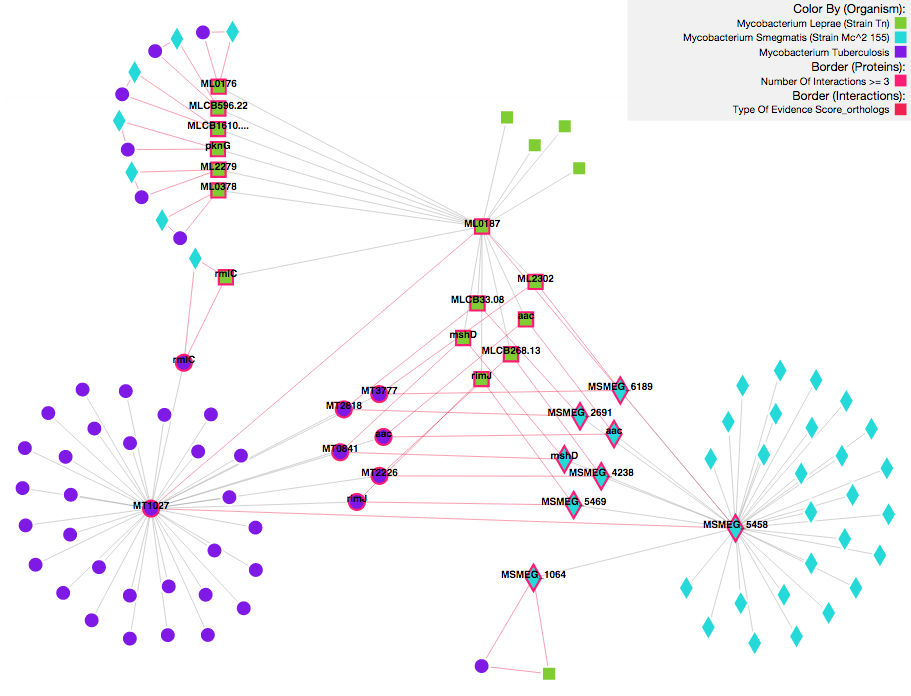
\includegraphics[width=\textwidth]{figures/pinv_orthologs.png}
\caption[Three ortholog proteins in MTB, MLP and MSM]{Three orthologs proteins in MTB, MLP and MSM: Q7D903, Q9CD64, A0R3F9 and their neighbours.
\label{fig:pinv_orthologs}}
\end{figure}

The interactive version of figure \ref{fig:pinv_orthologs} can be seen at \url{http://biosual.cbio.uct.ac.za/pinViewer.html?status=a512969c93f31b50926415e7fec14096.json}. This visualisation includes the different images used in the published article of this research \cite{AKI2013}, all of which were created using PINV.

\subsection{Impact on PINV}
This project was also carried out in the same research group where PINV was developed and the projects were executed simultaneously, which again allowed us to have first hand contact with the potential users of PINV while still in the design stages. As a consequence, some of the visualisation needs of this project influenced PINV development.

Firstly, this project required the display of three different species at a time, which made it evident that PINV should support the visualisation of interactions from multiple organisms. The  solution implemented in PINV was to visualise the proteins in the network using different SVG symbols for each organism,  meaning that PINV will automatically choose one symbol from those available when a protein from an organism that has not yet been displayed is added. Currently there are six available symbols, but the list can be extended in the future. Figure \ref{fig:pinv_orthologs} uses circles for MTB, squares for MLP and diamonds for MSM.

As a complement, we extended the force-directed layout, including selective gravity forces, attracting each organism's proteins to different points in the graphic, which helps to automatically separate the proteins and avoid cluttered areas of multiple species.

One characteristic specific to this project was the use of information of orthologs between species. We decided to include it in the dataset to be uploaded to PINV as another type of interaction, creating an extra evidence score column in the data. This allows the user to reuse all the functionalities defined for interactions. For example, the spring forces in the network view work the same with this pseudo-interaction, and as a result the orthologs are pulled out of the main group interactions of each organism. In figure \ref{fig:pinv_orthologs} for instance, the proteins that share orthologs in the other organisms have been pulled to the centre of the graphic, so they are easily identifiable.

\begin{figure}
\centering
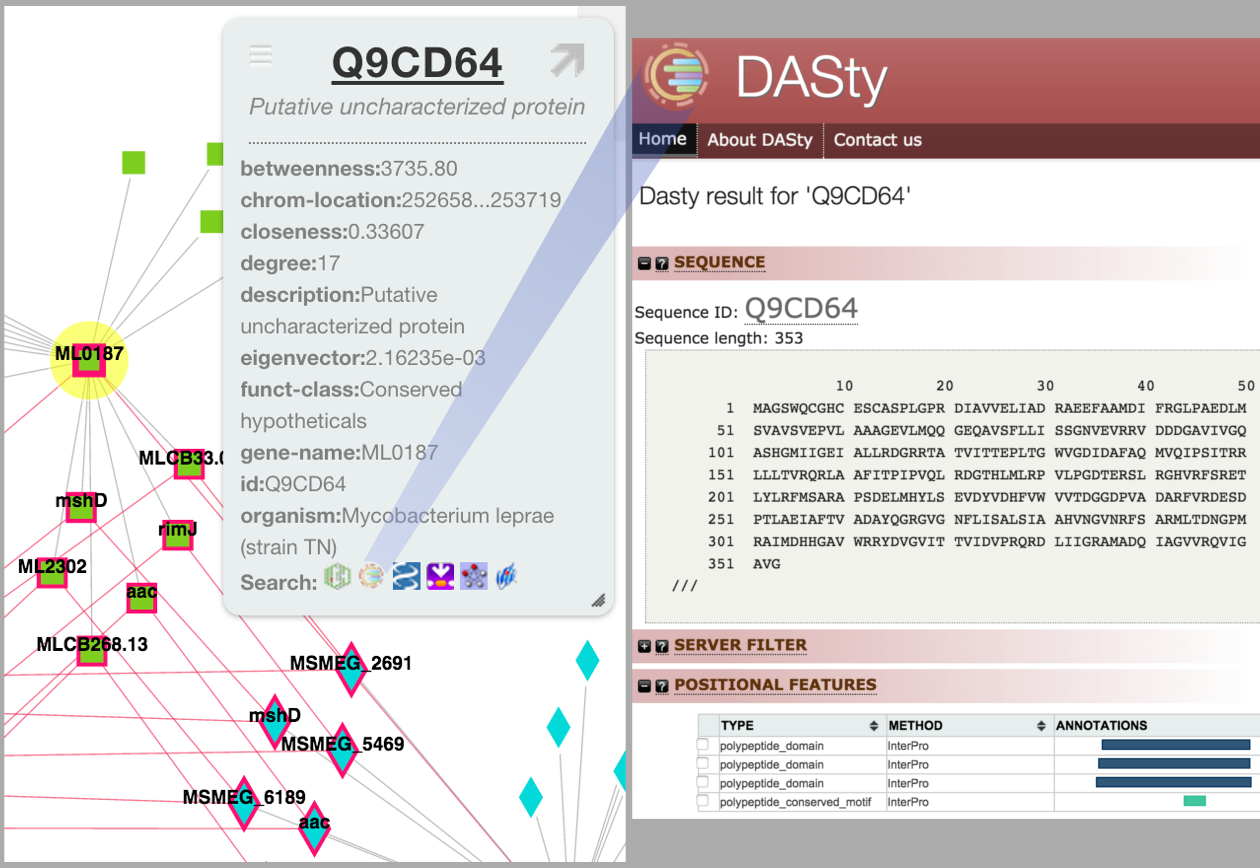
\includegraphics[width=5in]{figures/pinv2dasty.png}
\caption[Opening DASty3 from a protein of interest in PINV.]{Opening DASty3 from a protein of interest in PINV.
\label{fig:pinv2dasty}}
\end{figure}

Another requirement gathered during this collaboration was the need to link the proteins of interest to other resources outside the PINV dataset, and being able to gain access to more information. Figure \ref{fig:pinv2dasty} shows on the left hand side the popup window that is displayed when a protein is selected in PINV, and includes the features that were uploaded to the dataset by the user. In addition, PINV also shows links to several external resources at the bottom of the popup window, and for instance if the user clicks on the DASty3 logo, this application will open in another window with related information on the selected protein.


\section{Shotgun Analysis of Platelets From Patients Infected with the Dengue virus}
\label{sec:dengue}
\subsection{Research description}
In an attempt to better understand the phatogenesis of dengue virus infection, a group of researchers from the Brazilian foundation Fiocruz carried out a study to evaluate the impact of dengue infection on platelet activation. Their strategy was to compare the protein expression of healthy v.s. infected cells using label free mass spectrometry (publication in production).

Here, we describe a selection of the preliminary results and the techniques used during the project. More than three thousand proteins were identified in two conditions: healthy and infected with the dengue virus. From these, the results showed 619 proteins differentially expressed including those only present in one of the two conditions. The subset of differentially expressed proteins that are present in both groups contains 167 elements.

The identified proteins were then analysed in the context of their metabolic pathways by including information from the KEGG database. Similarly, the gene ontology (GO) annotations were used to enrich the dataset with biological functions.  Futhermore, a PPI network dataset was built using the protein interaction information reported in the STRING database.

In a first interaction analysis, all the differentially expressed proteins and the proteins detected in only one condition were included. Figure \ref{fig:pinv_platelets_1} represents the network, which has been colour coded to identify the class of differential expression: the proteins that were only expressed in patients infected with the dengue virus (light blue) and those that were only detected in the control patients (yellow) are indicated. For the expression data present in both groups, the under- (red) and over-expressed (green) proteins are shown.  

\begin{figure}
\centering
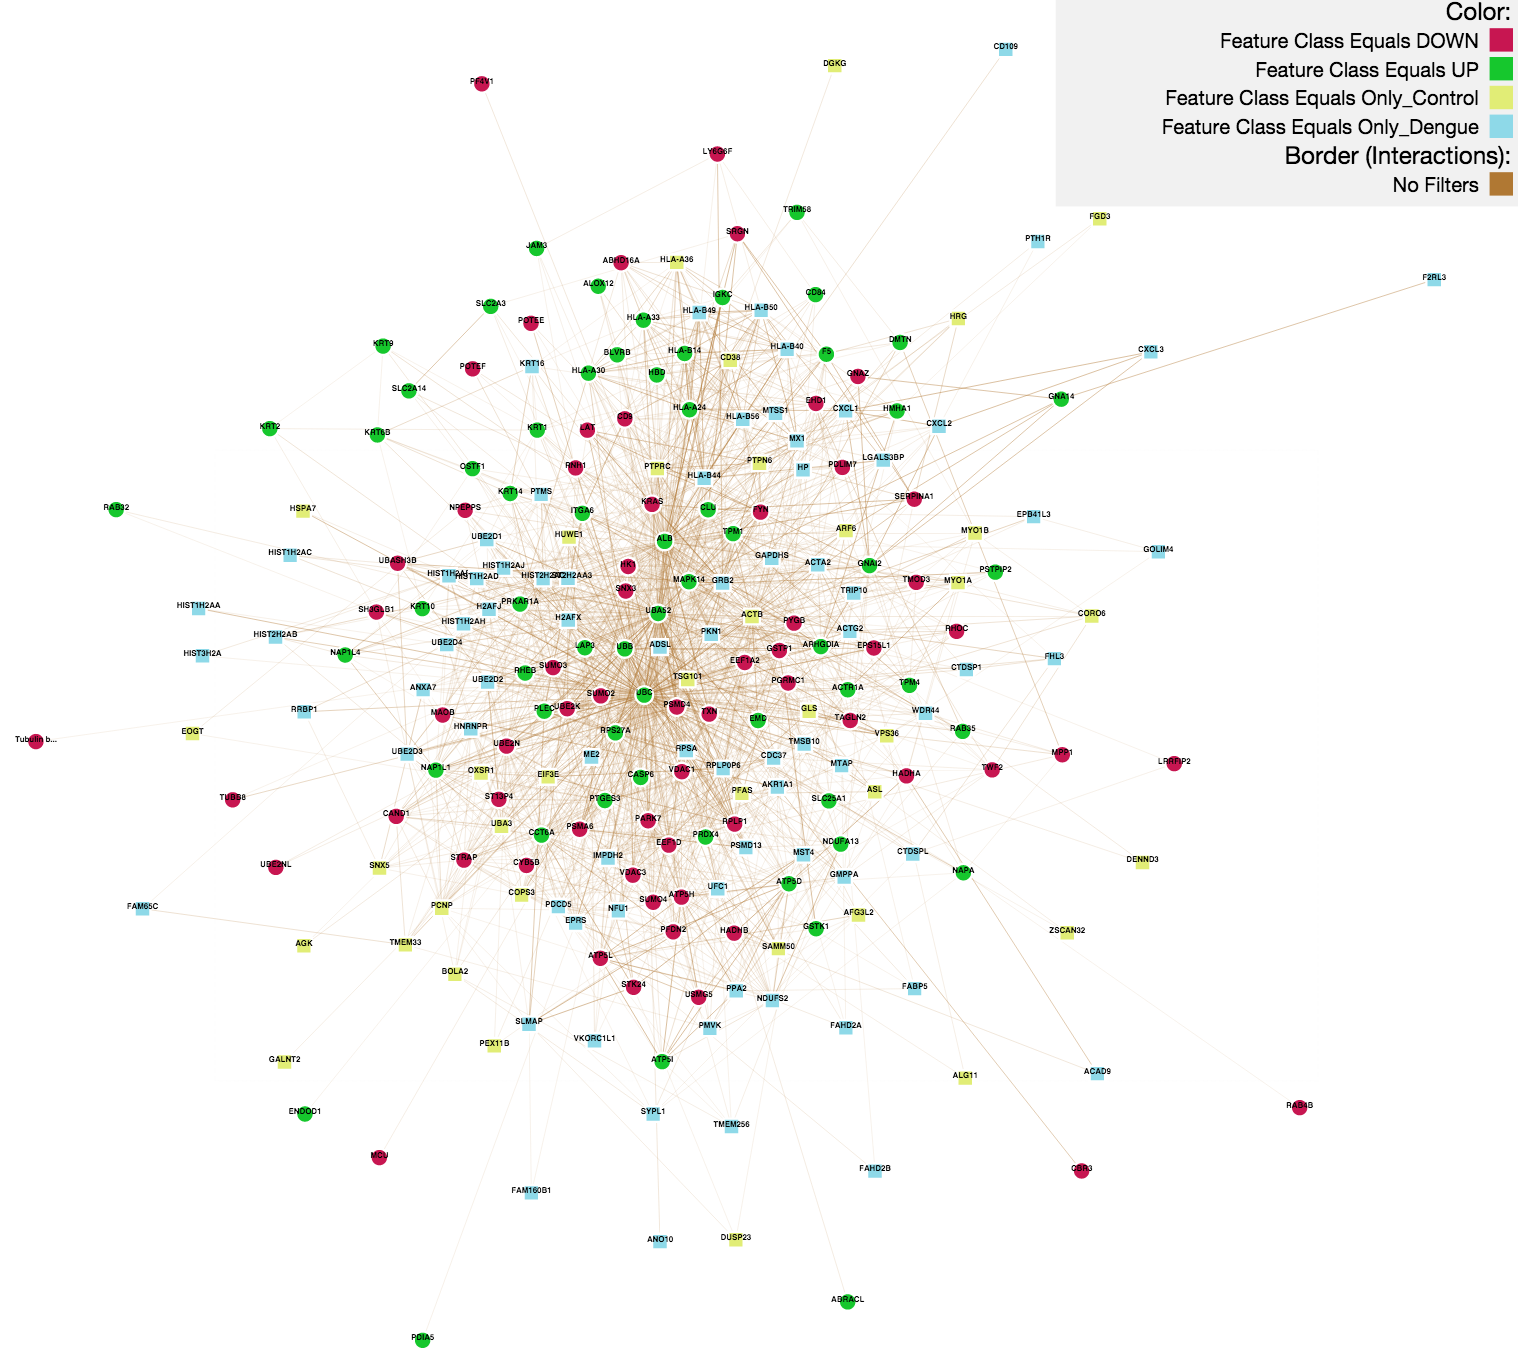
\includegraphics[width=\textwidth]{figures/pinv_platelets_1.png}
\caption[PPI network of differentially expressed platelets proteins in a dengue study.]{PPI network of differentially expressed platelets proteins in a dengue study.
\label{fig:pinv_platelets_1}}
\end{figure}

When the functional classes from GO were considered, it was found that the eight most statistically significant biological processes were related to ``antigen processing and presentation'' pathways, which indicates a potential role in the dengue pathological state. Some of these proteins are also related to proteasome/ubiquitinylation pathways.

To confirm whether these proteins interact directly with proteins related to the ``platelet activation'' pathway, a new graphic was created focusing on the specific non-redundant proteins involved in the ontology terms of interest. Figure \ref{fig:pinv_platelets_2} shows the subnetwork of interactions where at least one of the proteins was annotated with GO terms that contain the text: ``proteasome'', ``antigen'', ``platelet'' or ``mithocond''; colour coded in Figure \ref{fig:pinv_platelets_2} by yellow, red, blue, and pink, respectively.

\begin{figure}
\centering
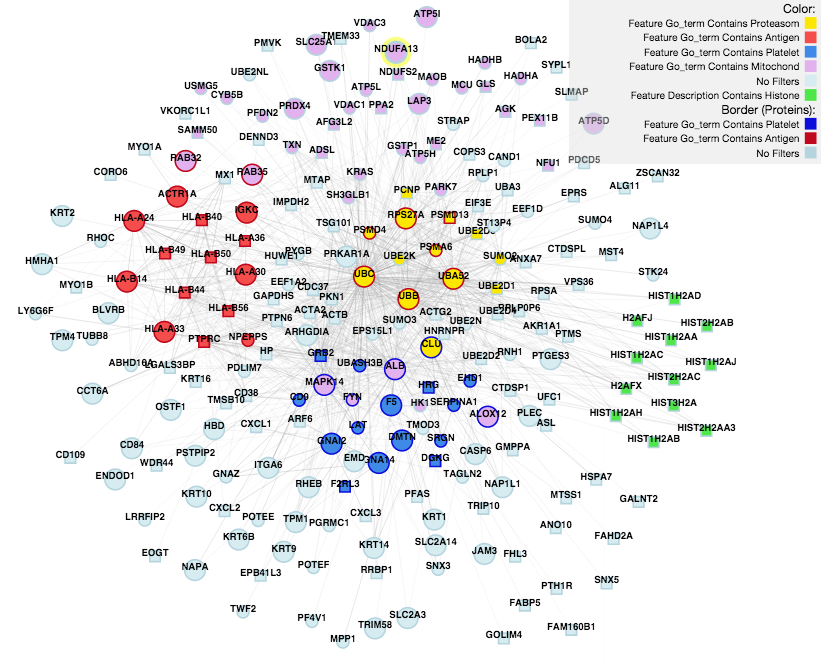
\includegraphics[width=\textwidth]{figures/pinv_platelets_2.png}
\caption[Subnetwork of the differentially expressed proteins identifying the most predominant GO terms.]{Subnetwork of the differential expressed proteins in the Dengue platelets dataset, identifying the most predominant GO terms by colour.
\label{fig:pinv_platelets_2}}
\end{figure}

\subsection{Impact on PINV}
We used PINV to assist the research group to create the network files and select an appropriate visualisation of their findings. The network was created using the reported interaction in STRING, which we filtered to include only the interactions between the proteins of interest, i.e. those which have been differentially expressed in the experiment. This required several preprocessing steps, including mapping of accession numbers between resources and the enrichment of the existing annotations with gene ontology data.

We have documented the step-by-step process in order to assist future researchers who have similar research requirements. The git repository in \url{https://github.com/4ndr01d3/pinv-server/tree/master/data-preparation} contains the script used to create the files, as well as explanations of the required file formats and logical thought processes behind the script.

The figures above were created using PINV; the web versions of these images are available at \url{http://biosual.cbio.uct.ac.za/pinViewer.html?status=67049496bf99027c6d6f3ba33a9cb77b.json} for Figure \ref{fig:pinv_platelets_1} and \url{http://biosual.cbio.uct.ac.za/pinViewer.html?status=c1f68787907a83e27fab70be329582ce.json} for Figure \ref{fig:pinv_platelets_2}.

The selection of these visualisations was a collaborative effort between researchers of both groups, in which our peers from the Brazilian laboratory led the process due to their knowledge on dengue viruses, whereas our contribution focussed on the computational aspects, including visualisation and PINV functionality.

The important collaborative features of PINV that were exploited during this research demonstrated the great value of the tool in assisting the communication between international groups. PINV as a native web tool that does not require installation of any software besides a modern browser. Moreover, PINV capability to reconstruct a specific network view from a generated URL, supported the communication between the researchers, allowing any individual to point out the features that one group considered either important or irrelevant for inclusion in a particular visualisation.

A specific example of the benefits of using PINV for the visualisation of the networks was exposed during this project: on a previous version of Figure \ref{fig:pinv_platelets_2}, we were not considering the GO terms related with mitochondrial processes, however while exploring the visualisation, an external collaborator pointed out that there were several proteins enriched with GO terms related to mitochondrial processes (e.g. mitochondrion, mitochondrial inner membrane, positive regulation of mitochondrial depolarization, mitochondrial matrix), which provided further insight and offered a future research hypothesis to determine the potential biological relevance of this mitochondrial association with dengue viral-infected platelet cells.

\section{Analysis of potential impact of SNPs on the human PPI network and gene expression}
\label{sec:pop_genetics}
\subsection{Research description}
This study investigated the impact of single nucleotide polymorphisms (SNPs) on human proteins particularly in the context of its protein-protein interaction network and taking into consideration gene expression for eight HapMap populations.

Previous studies have analysed the consequences of SNPs in different disease states \cite{BAU2009}. In several of these studies, attempts have been made to establish the relevance of the mutated protein in the human PPI network \cite{SAU2011}. Their findings suggest that there are diseases that are caused solely through the disrupted interactions. \emph{Heekes et al.}, extend these studies in order to consider SNPs that are located in non-coding regions as well as the differences in allele frequencies between populations \cite{HEE2014}.

The project's methodology starts by integrating data from multiple resources in the public domain: (i) human SNPs from NCBI (\url{ftp://ftp.ncbi.nlm.nih.gov/snp/organisms/human_9606_b141_GRCh37p13/VCF}), (ii) clinical related variations from ClinVar (\url{http://www.ncbi.nlm.nih.gov/variation/docs/human_variation_vcf/#clinvar}) and Humsavar (\url{http://www.uniprot.org/docs/humsavar})  (For the remainder of the document referred to as clinSNPs), (iii) population data for allele frequencies (AF) and linkage disequilibrium (LD) for eight populations from HapMap (\url{ftp://ftp.ncbi.nlm.nih.gov/hapmap}), (iv) gene expression data for the selected populations from Array Express (\url{http://www.ebi.ac.uk/arrayexpress/experiments/E-MTAB-264/}), (v) SNPs associated with gene expression levels reported in the publications \cite{STR2007}, \cite{LAP2013}, \cite{HAU2014} and \cite{WU2013}, and (vi) the Human PPI network compiled in the research described in the article \cite{RAP2013}.

Three centrality measurements were used to define the importance of each protein in the network: degree, betweenness and closeness. When analysing these values for proteins with non-synonymous SNPs (nsSNPs) in the human PPI network, the data showed that proteins containing nsSNPs have significantly lower centrality measures than proteins without nsSNPs. This is an indication that proteins with less interactions are less important for information flow, and, therefore, these proteins can tolerate an amino acid change without the mutation having a major impact on the network.

A similar centrality analysis was executed with the subset of proteins containing SNPs that have been identified as linked to disease states, and in this case it was shown that these proteins tended to have significantly higher centrality measures than non-mutated proteins. This can be explained by the implications on the structural changes caused by the mutation, which if it is considerable, might inhibit some of the established interactions. This is not critical for proteins with a small number of interactions, but for central proteins the effect can escalate to the level where the network collapses, and, hence, causes the disease.

The integrated dataset can be used to explore particular disease states and potentially improve the understanding of inter-population variation. An example was included in a research project where proteins with SNPs related to hypertension were selected, namely ADD1, NOS3, AGT and KCNMB1. Figure \ref{fig:pinv_human_snps} shows the subnetwork of these proteins that only display high confidence interactions (score ≥ 0.7), in which both of the proteins contained a nsSNP and at least one of the proteins contained a clinSNP  associated with hypertension. The figure is colour coded to highlight the significant differences in AF and gene expression between African populations. 

\begin{figure}
\centering
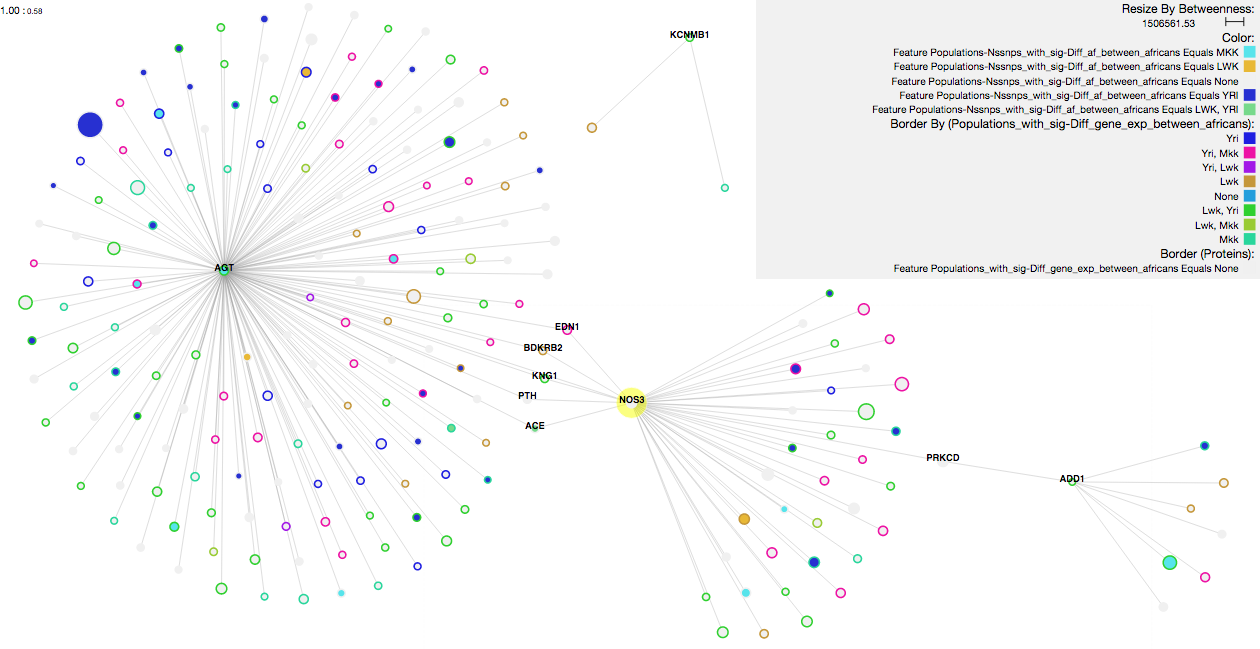
\includegraphics[width=\textwidth]{figures/pinv_human_snps.png}
\caption[Interactions between proteins with a hypertension clinSNP]{Interactions between proteins with a hypertension clinSNP and proteins with nsSNPs in the context of AF and gene expression differences between African populations.
\label{fig:pinv_human_snps}}
\end{figure}

Similar comparisons among other populations are included in \cite{HEE2014}, where the authors discuss the implications of the identified proteins in more detail. All the graphics were created using PINV. An interactive version of Figure \ref{fig:pinv_human_snps} is available at \url{http://biosual.cbio.uct.ac.za/pinViewer.html?status=dc029e8ef629cd4fed0c4a1509a70ef7.json}.

\subsection{Impact on PINV}
The case explained above, where hypertension-related proteins were analysed in the context of PPI networks, was carried out using only PINV. The dataset used during this research was uploaded to the PINV server, and is available under this URL: \url{http://biosual.cbio.uct.ac.za/pinViewer.html?core=HumanHapMapSNPs}. 

The authors were able to explore their data by defining different combinations of filters, for example, Figure \ref{fig:pinv_prefilters_snp} is a snapshot of the selected filters used for the generation of Figure \ref{fig:pinv_human_snps}, which we will describe from top to bottom: 
\begin{enumerate}
\setlength\itemsep{-0.5em}
\item This filters the whole human PPI network (1298519 interactions) in order to include only the proteins with high confidence interactions (score ≥ 0.7). This resulted in a total of 306453 interactions.
\item The second filter allows researchers to focus only on the interactions between proteins with nsSNPs. There are 182755 interactions in the whole network complying with this restriction, and in combination with the first filter, the subset is further reduced to 50211 interactions.
\item There is a total of 209540 interactions where at least one of the proteins has a SNP linked to a disease, and from this, 9662 interactions also pass the previous filters.
\item This filter selects all the interactions where at least one of the proteins contains the term ``\emph{hypertension}'' within a field where all the protein-specific diseases-causing SNPs are listed. In this way, 1711 interactions were found, and the intersection with the other filters produced 212 interactions.
\end{enumerate}

\begin{figure}
\centering
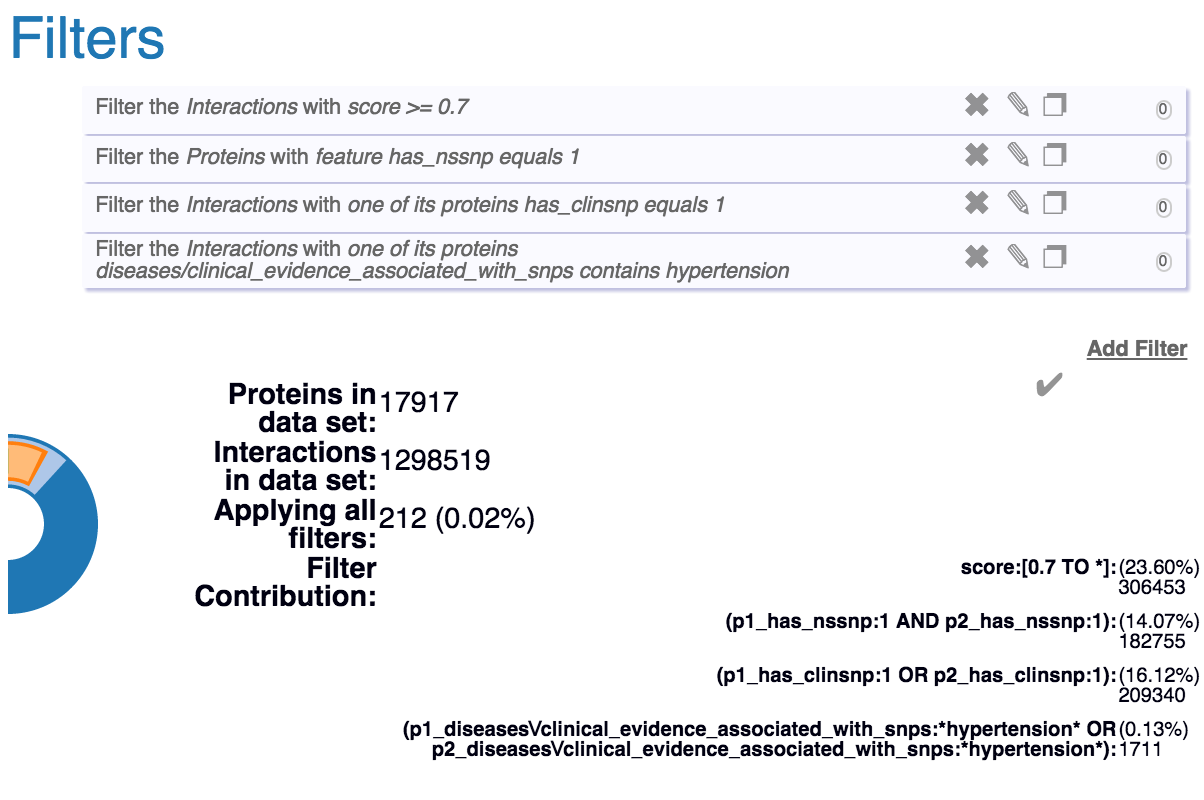
\includegraphics[width=5in]{figures/pinv_prefilters_snp.png}
\caption[Selection of filters for image \ref{fig:pinv_human_snps}]{Selection of filters for image \ref{fig:pinv_human_snps}
\label{fig:pinv_prefilters_snp}}
\end{figure}

From the resultant, final, graphic, only four proteins have been identified that are directly related to hypertension, and although it was not specifically imposed by the filters, the subnetwork connects three of the proteins with one degree of separation. This finding agrees with the notion that some disease states can be better understood by studying their associated proteins in the context of the human PPI network.

Once the network is identified, further factors can be analysed, for instance, the colour coding in Figure \ref{fig:pinv_human_snps} represents differently expressed proteins in different African populations. This may add to our understanding on why a disease affects populations in different ways. As part of our future goals, we plan to define a strategy for comparing networks that share the same structural features. This will allow us to compare, on a single graph, the network analysis for African populations \emph{v.s.} that of European or American populations. 

The example presented in this research demonstrates how PINV can be used for the exploration of PPI data, and how the use of filters supplies an alternative to navigate the data when the accession numbers of the proteins of interest are unknown. A similar protocol to that described above can be used to explore other clinical conditions, for instance, \cite{HEE2014} created a similar visualisation for proteins related to cancer. This is an example of how a publicly available dataset uploaded in PINV can benefit more than one research project or group.

During the entire project, the authors provided constant feedback and suggestions on how to improve PINV. For instance, several features related to uploading data, such as the sheer volume of data in certain experiments, were corrected or improved.

\section{Discussion}
In our view, the success of a software tool is highly dependent on the community that supports it.  This includes collaborators, developers and end users, all contributing in different ways to the continued growth of a tool. The described cases have contributed to the development of PINV in several ways, from reporting bugs and providing suggestions, to defining the core requirements of the tool. 

PINV has also benefited from articles and posters that include visualisations generated with the tool. It is clear that one of the main objectives for  a scientist is to explain his/her research in a clear, descriptive way, and thus, PINV provides several tools to facilitate this goal, and as a side effect, other researchers will be exposed to visualisations created with PINV, which increases its visibility to the right audience. 

\begin{figure}
\centering
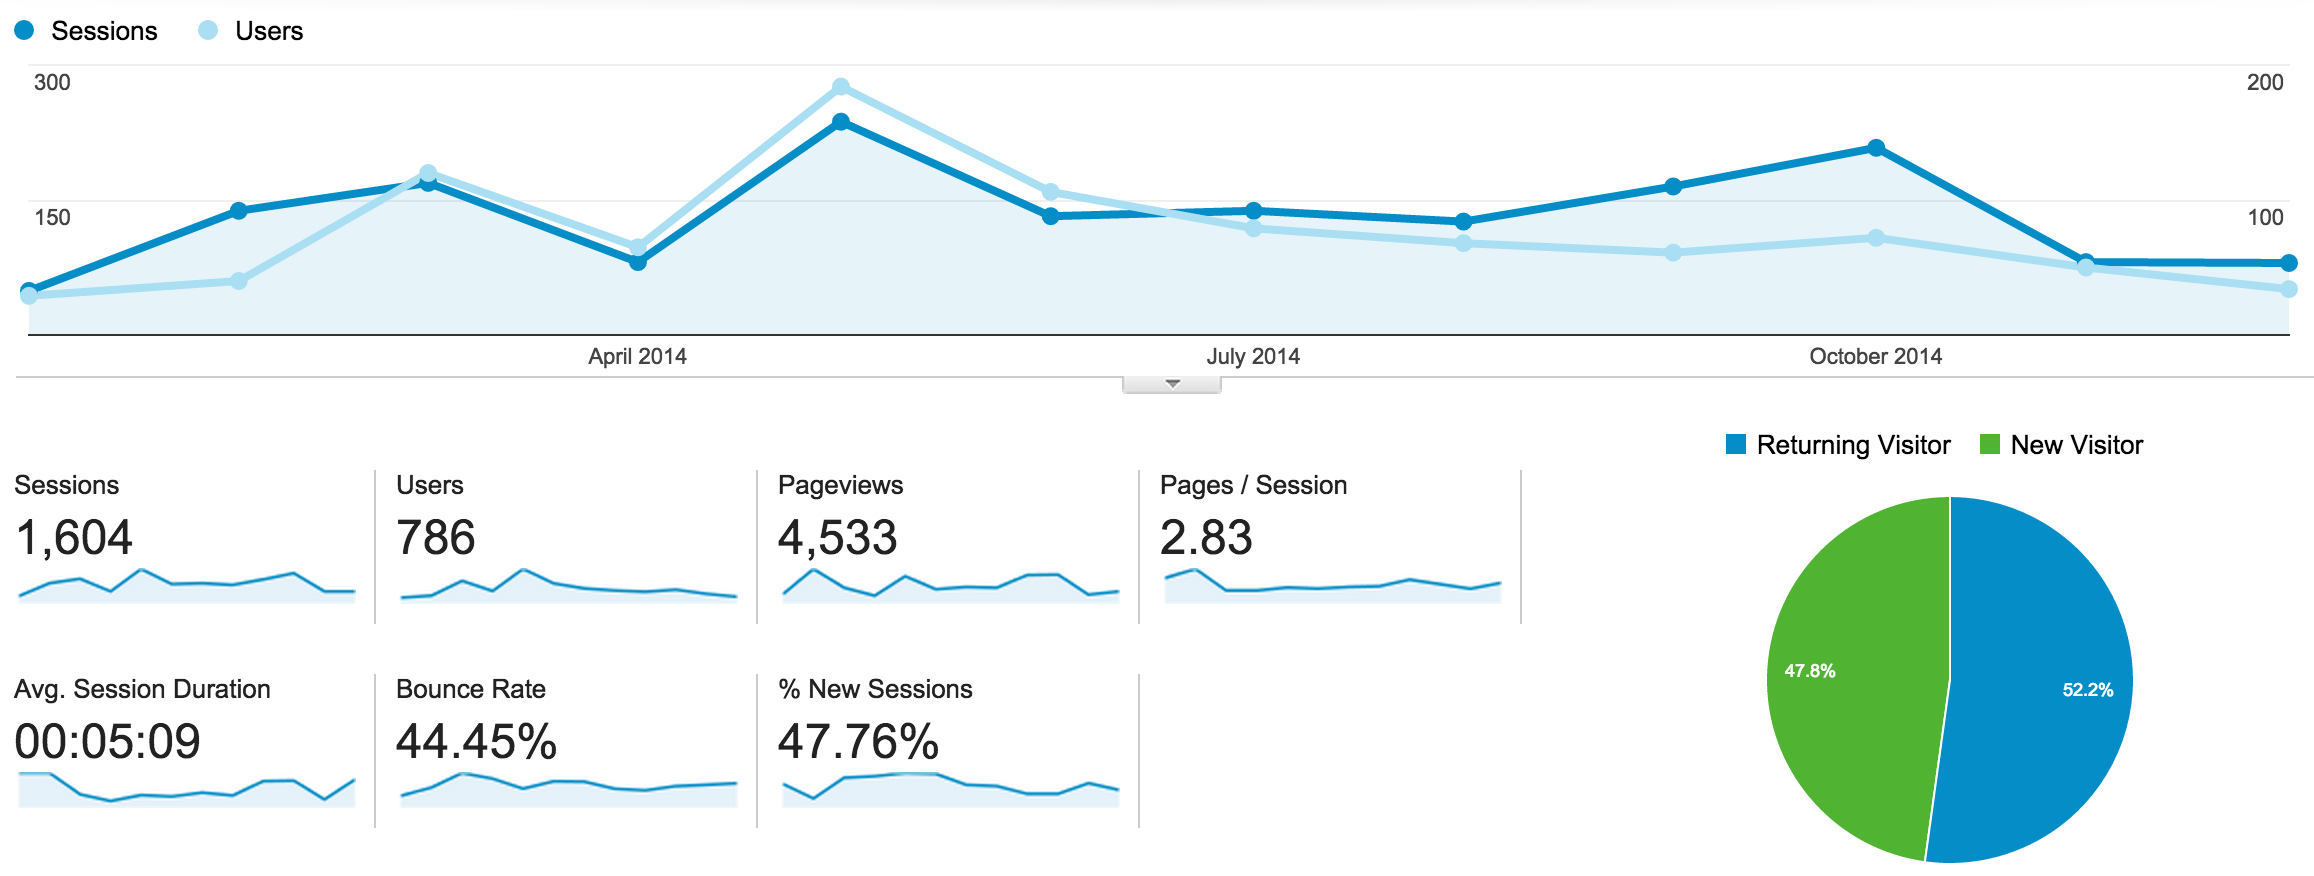
\includegraphics[width=\textwidth]{figures/google_analytics.png}
\caption[Usage statistics of PINV during 2014]{Usage statistics of PINV during 2014. 
\label{fig:google_analytics}}
\end{figure}

In order to track the usage of PINV, we are using google analytics (\url{https://www.google.com/analytics/}), and Figure \ref{fig:google_analytics} includes several graphics illustrating the recorded visits to the PINV's website during 2014. A total of 786 users visited the PINV url a total of 1604 times. From these sessions, 837 were registered as returning users, which we consider invaluable, as this suggests that returning users are working with PINV on a continued basis, and not only visiting the site out of curiosity.  Notwithstanding, we do not want to underestimate the importance of new visitors (767 recorded during 2014), since any returning user was once a new visitor.

The top graph in Figure \ref{fig:google_analytics} shows the number of sessions (blue) and users (light blue) per month. The first peak corresponds with the release of our scientific article \cite{SAL2014} and, therefore, likely illustrates the interest of the readers of the journal. The paper was tagged as \emph{Highly accessed} by the journal (BMC bioinformatics), and by April 2015 has been accessed 3041 times. The second highest peak in the graph, coincides with an oral presentation during the congress of the South African Society of Bioinformatics; the talk was awarded the best PhD presentation prize at the conference.

PINV is a young and highly specialised tool and we therefore do not expect the site visit and usage statistics to compare with that of  well known web sites, such as \url{www.google.com} and \url{www.wikipedia.org}, which generate millions of hits per day. However, we are motivated by the enthusiasm from the currently small target audience and are confident that PINV will facilitate, and contribute to, the research of scientists focussing on protein-protein interactions.
